\documentclass[11pt]{report}

\usepackage[T1]{fontenc}
\usepackage[polish]{babel}
\usepackage[utf8]{inputenc}
\usepackage{lmodern}
\usepackage[pdftex]{graphicx}
\selectlanguage{polish}
\usepackage{amsmath}
\usepackage[top=3cm, bottom=3cm, left=3cm, right=3cm]{geometry}
\usepackage{algorithm,algorithmic}
\title{System do automatyzacji procesu składania planu zajęć z wykorzystaniem algorytmów genetycznych}

\begin{document}

%
% przeczytaj: http://en.wikibooks.org/wiki/LaTeX/Document_Structure
%

\maketitle
\tableofcontents


\chapter{Wstęp}

\section{Kontekst zagadnienia}
\textit{Katarzyna Śmietanka}
\par Problem układania planu zajęć dotyczy wielu instytucji głównie związanych ze szkolnictwem, od szkoły podstawowej aż do szkół wyższych. Zadanie sprowadza się do przygotowania graficznego rozkładu zajęć: dla poszczególnych klas - uczniów uczęszczających do danej klasy, planu zajęć dla każdego z uczących nauczycieli oraz rozkładu zajęć odbywających się w poszczególnych salach. Układanie planów zajęć nawet dla niewielkiej szkoły wymaga dużego wysiłku oraz nakładu czasowego. Problem staje jeszcze bardziej skomplikowany dla szkół ponadgimnazjalnych, do których uczęszcza więcej uczniów a tym samym jest więcej klas, nauczycieli oraz realizowanych przedmiotów. Ponadto, istnieje wiele wariantów tego problemu; na niektórych uczelniach, gdzie studenci sami mogą wybierać zajęcia, złożoność problemu jest o wiele większa. Trudność problemu związana jest z podstawowymi kryteriami, które musi spełniać plan zajęć aby był właściwy: dwa różne zajęcia, na które zapisany jest minimum jeden student nie mogą się odbywać w tym samym czasie, dwa różne zajęcia w tym samym czasie nie mogą odbywać się w tej samej sali oraz nauczyciel w danym momencie może nauczać tylko jednego przedmiotu. Rozszerzeń tych ograniczeń jest wiele, a uwzględnienie każdego z nich, często konieczne do stworzenia realnego planu zajęć jest niezbędne. Wprowadzanie kolejnych ograniczeń znacznie utrudnia problem, który i tak jest stosunkowo skomplikowany.
\par Pomysł tematu pracy inżynierskiej wyniknął z przyglądania się na przestrzeni naszej edukacji planom zajęć, które często odbiegały od idealnego według naszej opinii. Plan zajęć często zawierał sporo przerw między obowiązkowymi zajęciami, zajęcia zaczynały się bardzo wcześnie lub kończyły bardzo późno, co w znacznym stopniu utrudniało powrót do domu bądź też dopasowanie innych pozauczelnianych zajęć do naszego planu.
\par Problem ułożenia planu zajęć podejmowany był w wielu pracach naukowych również na Politechnice Gdańskiej, co świadczy o tym że ułożenie bezkonfliktowego planu zajęć jest problemem stosunkowo trudnym do rozwiązania a zarazem bardzo ciekawym, ponieważ w bezpośredni sposób dotyczy każdej uczącej się osoby. Dlatego też na przestrzeni wielu lat powstało wiele różnych podejść do tego problemu od algorytmów klasycznych poprzez różnego typu algorytmy sztucznej inteligencji.
\par Problem układania graficznych rozkładów nie tylko związany jest ze szkolnictwem, ale również dotyczy układania rozkładów jazdy komunikacji miejskiej \cite{com}, planu zajęć dla pracowników \cite{worker} oraz terminarza zawodów sportowych \cite{sport}.
\section{Cel}
\par Celem naszej pracy jest stworzenie systemu do automatyzacji procesu układania planów zajęć z wykorzystaniem Algorytmu Genetycznego (Genetic Algorithm).  W przeciągu ostatnich lat pojawiły się nowe podejścia, algotymy rozwiązujące problem układania planu zajęć, które postawiły algorytm genetyczny w nowym świetle. Chęć głębszego zapoznania się z postawionym przed nami problemem sprawiła, że zdecydowaliśmy się na rozszerzenie zagadnienia tematu naszej pracy inżynierskiej o kolejne implementacje algorytmów: Algorytm Roju Cząsteczek (Particle Swarm Optimization) oraz Algorytm Adaptacyjny Tabu (Adaptive Tabu Search). Ponadto w celu urzeczywistnienia problemu zdecydowaliśmy się na przystosowanie działania naszych algorytmów do realych danych, uzyskanych z jednej z gdyńskich szkół ponadgimnazjalnych.
\par Implementacja algorytmów: Genetycznego, Roju Cząsteczek oraz Adaptacyjnego Tabu postawiła nas przed ciekawą możliwością porównania działania tych algorytmów, co jak się okazuje nie jest łatwym zadaniem.
\section{Zakres pracy}
\par Na realizację postawionego celu składa się:
\begin{enumerate}
\item System do automatyzacji procesu układania planu zajęć
\begin{enumerate}
\item Frontend — aplikacja kliencka, odpowiadająca za interakcję z użytkownikiem: wprowadzanie danych wejściowych, wybór algorytmu do generowania planu zajęć oraz wizualizacja wygenerowanego planu zajęc w Ext JS Calendar.
\item Backend - generowanie planu zajęć z danych prowadzonych przez użytkownika 
\end{enumerate}
\item Implementacja algorytmów
\begin{enumerate}
\item Algorytm Genetyczny
\item Algorytm Roju Cząsteczek
\item Algorytm Adaptacyjny Tabu
\end{enumerate}
\item Przetworzenie danych szkolnych do zaimplementowanych algorytmów
\item Porównanie działania algorytmów

\end{enumerate}


\section{Podział zadań i obowiązków}
\begin{enumerate}
\item Tomasz Dziopa 
\begin{itemize}
\item Implementacja Algorytmu Adaptacyjnego Tabu
\item Przystosowanie działania algorytmu (ATS) do danych szkolnych
\item Implementacja systemu do automatyzacji procesu układania planów zajęć: stworzenie interfejsu użytkownika, wizualizacja wygenerowanych planów w Ext JS Calendar
\end{itemize}
\item Paweł Jastrzębski
\begin{itemize}
\item Implementacja Algorytmu Roju Cząsteczek
\item Implementacja systemu do automatyzacji procesu układania planów zajęć: stworzenie formularza do dodawania zadań, list do wyświetlania zadań, zdalne uruchamianie zadań poprzez rozproszoną kolejkę 
\end{itemize}
\item Filip Czajkowski
\begin{itemize}
\item Implementacja Algorytmu Genetycznego
\item Przystosowanie działania algorytmu (GA) do danych szkolnych
\item Przygotowanie dokumentacji dla Systemu do automatyzacji procesu układania planów zajęć
\end{itemize}
\item Katarzyna Śmietanka
\begin{itemize}
\item Implementacja Algorytmu Adaptacyjnego
\item Przystosowanie działania algorytmu (ATS) do danych szkolnych
\item Przetworzenie danych szkolnych do struktury zaimplementowanych algorytmów
\item Porównanie działania algorytmów, przygotowanie wizualizacji danych wejściowych
\end{itemize}
\end{enumerate}
\section{Środowisko pracy i narzędzia}
\paragraph{} Przy tworzeniu pracy inżynierskiej korzystaliśmy z repozytorium git w serwisie github.com \cite{github} z podpiętym narzędziem typu \textit{continuous integration} o nazwie travis \cite{travis}. Praktycznie cały kod został napisany w języku Python w wersji interpretera 2.7.6. Do testów jednostkowych użyto modułu \verb#nosetests#, aplikacja webowa została oparta o framework \verb#django# w wersji 1.6 i rozproszoną kolejkę zadań \verb#celery# \cite{celery}.
\paragraph{} 
\chapter{Opis problemu układania planu zajęć}


\chapter{Specyfikacja problemu}
\textit{Filip Czajkowski, Katarzyna Śmietanka} \\
\paragraph{}Specyfikacja problemu układania planu zajęć różni się bardzo w kontekście konkretnego przypadku. Dlatego też chcieliśmy, aby nasze implementacje opierały się na dobrze opisanym przypadku, który umożliwi jasne określenie wymagań względem naszych rozwiązań i pozwoli na ich jednoznaczne porównanie. Okazało się, że odbywający się co kilka lat międzynarodowy konkurs na najlepsze rozwiązanie w tej dziedzinie bardzo dobrze spełnia te założenia.
\section{International Timetabling Competition 2007}
\textit{Filip Czajkowski} \\
\subsection{Opis konkursu}
\paragraph{International Timetabling Competition (ITC)}\cite{itc} to międzynarodowy konkurs w dziedzinie układania planów zajęć organizowany przez międzynarodowe środowisko akademickie. Jego celem jest lepsze poznanie problemu rozkładania zajęć lub egzaminów na uczelni, z którym zmagają się od bardzo dawna i wciąż potrzebują stosowania lepszych rozwiązań. W 2007 roku odbyła się jego druga edycja, w której można było startować w dowolnej z trzech kategorii: 
\begin{itemize}
\item Układanie rozkładu sesji egzaminacyjnej na uczelni. W tym przypadku zakłada się, że wszyscy studenci zapisani na swoje zajęcia muszą mieć możliwość wzięcia udziału we wszystkich dotyczących ich egzaminach. Plan powstaje zatem po zapisaniu się wszystkich studentów na wybrane przez siebie przedmioty.
\item Tworzenie planu zajęć dla studentów zapisanych na konkretne zajęcia. W tym przypadku rozkład wszystkich zajęć obowiązujących przez cały semestr jest generowany w momencie, gdy studenci wybrali już przedmioty, na które zajęcia chcą uczęszczać. Ten model rozwiązania jest dostosowany do elastycznych programów nauczania, które uczelnie coraz częściej stosują.
\item Układanie planu zajęć dla każdego planu nauczania. Tworzony jest tygodniowy rozkład lekcji, które są przyporządkowane do poszczególnych programów nauczania, a także muszą spełniać ograniczenia czasowe narzucone przez władze uczelni. Udostępnione przykładowe dane przedmiotów, sal oraz wykładowców pochodzą z Uniwersytetu Udine we Włoszech.
\end{itemize}
W przewidzianym przedziale czasowym można było nadsyłać rozwiązania, które można było testować na części udostępnionych zestawach danych. Niedozwolone było stosowanie zrównoleglenia obliczeń w stosowanych rozwiązaniach. Ostatecznie, zwycięzcy w każdej z kategorii zostali ogłoszeni podczas konferencji w Montrealu w 2008 roku i każdy z nich otrzymał nagrodę pieniężną w wysokości 500\pounds .
\subsection{Konkurs a praca inżynierska}
\par Poszukując informacji o implementowanych przez nas algorytmach optymalizacyjnych w kontekście układania planu zajęć, natknęliśmy się na informacje o konkursie ITC w 2007 roku. Wspólnie stwierdziliśmy, że skorzystanie ze zdefiniowanych w nim ograniczeń i wymagań względem generowanego planu a także określona funkcja oceny rozwiązania bardzo pomoże nam zaprojektować nasze algorytmy oraz jednoznacznie je porównać. Nasze implementacje były tworzone pod kątem trzeciej kategorii konkursu, czyli rozkładu zajęć przedmiotów zawierających się we wcześniej zdefiniowanych programach nauczania.
\section{Sformułowanie problemu}

Celem jest stworzenie tygodniowego harmonogramu wykładów dla kilku kursów, z określoną liczbą dostępnych sal i przedziałów czasowych, w których mogą odbywać się zajęcia. Każdy wykład będący w programie danego kursu musi być przypisany do określonego przedziału czasu i sali tak by spełniał wejściowe ograniczenia. 
\subsection{Jednostki problemu}
\begin{itemize}
\item{\textbf{Dni, przedziały, okresy} - dzień podzielony jest na określoną liczbę przedziałów czasowych, okres para złożona z dnia i przedziału czasowego.}
\item{\textbf{Kursy i wykładowcy} - każdy kurs składa się z określonej liczby zajęć, które muszą być rozłożone w różnym czasie, na które uczęszcza określona liczna studentów i prowadzone są one przez konkretnego wykładowcę. Dla każdego kursu określona jest minimalna liczba dni, na które powinny być rozłożone zajęcia oraz okresy w których dane wykłady (zajęcia) nie mogą się odbywać.}
\item{\textbf{Sale wykładowe} - sale wykładowe mają ograniczoną liczbę dostępnych miejsc w pomieszczeniu.}
\item{\textbf{Program nauczania} - składa się z kilku kursów, na które uczęszcza grupa studentów.}
\end{itemize}
\subsection{Ograniczenia}
\subsubsection{Ograniczenia twarde}
Plan jest wykonywalny - czyli możliwy do realizacji, jeżeli żadne z wymienionych poniżej ograniczeń nie jest naruszone.
\begin{itemize}
\item  ${H_{1}}$ \textbf{Wykłady} - każdy kurs wchodzący w skład programu nauczania musi być przypisany do różnego okresu.
\item  ${H_{2}}$ \textbf{Zajętość sali} - żadne dwa wykłady nie mogą odbywać się w tym samym okresie w jednym pomieszczeniu.
\item  ${H_{3}}$ \textbf{Konflikty pomiędzy kursami} - zajęcia z tego samego programu nauczania bądź nauczanie przez tego samego wykładowcę muszą odbywać się w różnym czasie.
\item  ${H_{4}}$ \textbf{Dostępność wykładowcy} - zajęcia nie mogą się odbywać w czasie, w którym dany wykładowca nie może prowadzić zajęć.
\item ${H_{5}}$ \textbf{Typ sali} - każde z zajęć powinno odbywać się w odpowiedniej sali przystosowanej do przeprowadzania zajęć (odpowiednim typie sali) [*] - ograniczenie to dotyczy tylko $Szkolne\ dane\ wejściowe$
\end{itemize}
\subsubsection{Ograniczenia miękkie}
Ograniczenia te w bezpośredni sposób nie wpływają na wykonywalność planu zajęć, ale na jakość wygenerowanego planu zajęć, określoną na podstawie funkcji oceny.
\begin{itemize}
\item  ${S_{1}}$ \textbf{Wielkość sali} - liczba studentów uczęszczających na zajęcia w danej sali musi być mniejsza bądź równa liczbie dostępnych miejsc.
\item  ${S_{2}}$ \textbf{Stabilność pomieszczenia} - zajęcia wchodzące w skład jednego kursu powinny odbywać się w jednej tej samej sali, jeżeli jest to niemożliwe liczba sal w których odbywają się te zajęcia powinna być jak najmniejsza.
\item  ${S_{3}}$ \textbf{Minimalna liczba dni} - minimalna liczba dni na które powinny być rozłożone zajęcia z danego kursu.
\item  ${S_{4}}$ \textbf{Zwartość zajęć} - zajęcia wchodzące w skład jednego programu nauczania powinny odbywać się w jak najmniejszych odstępach czasowych między sobą. [*] - dotyczy to tylko $Danych\ konkursowych$
\end{itemize}
\subsection{Funkcja oceny - dla danych konkursowych}
\label{funkcjaOceny}
\textbf{Ograniczenia twarde} - podczas oceny końcowej wygenerowanego planu zajęć zliczane są poszczególne naruszenia ograniczeń twardych:\\
\begin{enumerate}
\item \textbf{Zajęcia / Wykłady} - naruszenie występuje w przypadku gdy zajęcia nie są przypisane do planu zajęć
\item \textbf{Zajętość sali} - naruszenie występuje gdy zostaną przypisane więcej niż jedne zajęcia do sali w tym samym czasie
\item \textbf{Konflikty} - naruszenie wystąpi wtedy, gdy dwa zajęcia będące w konflikcie odbywają się w tym samym czasie (tzn. ci sami studenci uczęszczają na te zajęcia lub prowadzone są przez tego samego wykładowcę)
\item \textbf{Dostępność} - naruszenie występuje gdy zajęcia odbywają się w czasie, w którym niedostępny jest wykładowca 
\end{enumerate} 

\textbf{Ograniczenia miękkie} - zliczanie punktów kary
\begin{enumerate}
\item \textbf{Wielkość sali} - Jeżeli liczba studentów jest większa niż liczba dostępnych miejsc w sali to za każdego dodatkowego studenta punkt kary pomnożony przez współczynnik ${a_{1} = 1}$ 
\item \textbf{Minimalna liczba dni}
Jeżeli liczba dni podczas których odbywają się zajęcia jest mniejsza niż minimalna liczba dni, podczas których powinny odbywać się zajęcia to do kary doliczamy różnicę między minimalną liczbą dni a liczbą dni, w których zajęcia się odbywają pomnożoną o współczynnik $a_{2} = 5$ 
\item \textbf{Zwartość zajęć}
Za każde zajęcia w planie, które nie przylegają do żadnych innych zajęć z tego samego programu nauczania, punkt kary pomnożony o współczynnik ${a_{3} = 2}$
\item \textbf{Stabilność pomieszczenia}
Te same zajęcia powinny odbywać się w jak najmniejszej liczbie różnych pomieszczań, za każde nowe pomieszczenie punkt kary pomnożony o współczynnik ${a_{4} = 1}$
\end{enumerate}

\subsection{Matematyczny zapis przestrzeni rozwiązań} \cite{tabu}
\par Na problem składa się ${n}$ kursów ${C = \{c_{1}, c_{2},...,c_{n}\}}$ które powinny być przydzielone do ${p}$ różnych okresów ${T = \{t_{1}, t_{2},...,t_{p}\}}$ oraz ${m}$ pomieszczeń w których mogą odbywać się zajęcia ${R = \{r_{1}, r_{2},...,r_{m}\}}$. Okres jest to para składająca się z dnia i przedziału czasowego (${d}$ - liczba dni a ${h}$ - liczba dziennych przedziałów czasowych, czyli ${p = d * h}$). Każdy z kursów składa się z ${n}$ zajęć ${L = \{l_{1},l_{2},...,l_{n}\}}$. Kursy wchodzą w skład ${s}$ programów nauczania ${CR = \{cr_{1}, cr_{2}, ..., cr_{s}\}}$, na program nauczania składają się kursy, na które uczęszczają ci sami studenci. 

\section{Dane wejściowe}
\label{sec:input_format}
\subsection{Konkursowe dane wejściowe}
\par Dane wejściowe zostały uzyskane z konkursu International Timetabling Competition 2007
\par Dane wejściowe są plikami tekstowymi, w których zawarte są ogólne informacje takie jak: liczba kursów, liczba dostępnych pomieszczeń, liczba dni na które mają być rozłożone zajęcia, liczba programów nauczania oraz ograniczenia precyzujące w jakich terminach nie mogą odbywać się zajęcia z danego kursu. Kolejno sprecyzowane są kursy, pomieszczenia, programy nauczania oraz ograniczenia w zadanym poniżej formacie:
\begin{verbatim}
Kursy: <Id Kurs> <Nauczyciel> <Liczba zajęć> <Minimalna liczba dni> <liczba studentów>
Sale: <Id Sala> <Pojemność sali>
Program nauczania: <Id Program Nauczania> <Liczba Kursów> <Ids Kursy>
Ograniczenia: <Id Kurs> <Dzień> <Okres>
\end{verbatim}
\begin{enumerate}
\item Każdy z kursów z danych wejściowych zawiera unikalny identyfikator, liczbę zajęć, która musi się odbyć w ramach tego kursu, minimalną liczbę dni oraz liczbę studentów, którzy uczęszczają na te zajęcia. 
\item Sale zawierają unikalny identyfikator oraz informację o maksymalnej liczbie studentów, która się zmieści w sali.
\item Na program nauczania składa się określona liczba kursów, których identyfikatory zawarte są w opisie programu nauczania  \verb#<Ids Kursy>#

\item W ramach ograniczeń umieszczona jest informacja o kursie \verb#<Id Kurs>#
 który nie może odbyć się w danym dniu w danym okresie.
\end{enumerate}
\subsection{Szkolne dane wejściowe}
\par Dane z roku szkolnego 2013/2014 uzyskane z jednej ze szkół gdyńskich ponadgimnazjalnych, która jest połączeniem szkoły zawodowej, technikum oraz liceum.
\par Dane zostały przystosowane do formatu ,,Konkursowych danych wejściowych'' rozszerzając je o pojęcie typu sali. Szczegółowy proces przetworzenia danych został opisany w sekcji ,,Etapy przetwarzania danych szkolnych''.
\begin{verbatim}
Kursy: <Id Kurs> <Nauczyciel> <Liczba zajęć> <Minimalna liczba dni> 
	   <liczba studentów><Typ sali>
Sale: <Id Sala> <Pojemność sali> <Typ sali>
Program nauczania: <Id Program Nauczania> <Liczba Kursów> <Ids Kursy>
Ograniczenia: <Id Kurs> <Dzień> <Okres>
\end{verbatim}
Rozszerzenie formatu danych wejściowych:
\begin{enumerate}
\item Wprowadzono \verb#<Typ sali>#, który przyjmuje poniżej zdefiniowane wartości:
\begin{verbatim}
n - zwykła sala lekcyjna
w - sala warsztatowa
l - biblioteka
o - poza szkołą
e - sala gimnastyczna / boisko szkolne / basen 
c - sala laboratoryjna (komputerowa)
\end{verbatim}
\item Został wprowadzony \verb#<Typ sali># dla każdego z kursów określający w jakich rodzajach sal mogą odbywać się zajęcia z tego kursu.
\end{enumerate}


\chapter{Opis zrealizowanych algorytmów}

\section{Adaptive tabu search (ATS)}
\textit{Katarzyna Śmietanka, Tomasz Dziopa}
\subsection{Rozszerzenie sformułowania problemu }
Rozszerzenie specyfikacji problemu z sekcji 3.2.4.
\par Problem definiujemy w postaci macierzy ${X}$  rozmiaru ${p \times m}$ gdzie ${x_{i,j}}$ ($x$ - unikalna etykieta zajęć) oznacza przypisanie danych zajęć do ${t_{j}}$ okresu oraz sali ${r_{i}}$. Jeżeli w danym czasie w danej sali nie odbywają się zajęcia wartość ${x_{i,j}}$ będzie przyjmowała wartość ${null}$. Dzięki takiemu sposobowi zdefiniowania problemu nigdy nie zostanie naruszone ograniczenie twarde ${H_{2}}$ dotyczące zajętości sali.

\begin{table}[H]
\begin{center}

\begin{tabular}{ r|c|c|c|c|c| }
\multicolumn{1}{r}{}
 &  \multicolumn{1}{c}{$r_{1}$}
 & \multicolumn{1}{c}{$r_{2}$} 
 & \multicolumn{1}{c}{$r_{3}$} 
 & \multicolumn{1}{c}{$...$} 
 & \multicolumn{1}{c}{$r_{m}$} 
 \\
\cline{2-6}
$t_{1}$ & $null$ & $matematyka$ & $biologia$ & $...$ & $geografia$ \\
\cline{2-6}
$t_{2}$ & $fizyka$ & $null$  & $null$ & $...$ & $religia$\\
\cline{2-6}
$t_{3}$ & $historia$ & $null$  & $null$ & $...$ & $null$\\
\cline{2-6}
$...$ & $...$ & $...$ & $...$ & $...$ & $...$ \\
\cline{2-6}
$t_{p}$ & $null$ & $matematyka$ & $chemia$ & $...$ & $fizyka$ \\
\cline{2-6}
\end{tabular}
\end{center}
\caption {Reprezentacja problemu w postaci macierzy $X$}
\end{table} 
\begin{itemize}
 \item Komórka $(t_{2}, r_{2}) = null$ w macierzy $X$ oznacza, że w czasie $t_{2}$ w sali $r_{2}$ nie odbywają się żadne zajęcia.
 \item Komórka $(t_{3}, r_{1}) = historia$ w macierzy $X$ oznacza, że w czasie $t_{3}$ w sali $r_{1}$ odbywają się zajęcia z przedmiotu $historia$.
\end{itemize}


\subsection{Ogólny opis algorytmu}
\label{ats_description}
\par Opis zaimplementowanego przez nas algorytmu został zaczerpnięty z pracy ,,Adaptive TabuSearch for Course Timetabling'' \cite{tabu}
\par Na całość algorytmu składają się trzy fazy. Najpierw w fazie inicjalizacji tworzony jest początkowy plan zajęć, przy pomocy zachłannej heurystyki. Następnie wykonywane są naprzemiennie fazy intensyfikacji i dywersyfikacji. W fazie intensyfikacji staramy się minimalizować funkcję oceny, natomiast w fazie dywersyfikacji poprzez operator zaburzeń nieco zmniejszamy jakość naszego rozwiązania, w celu opuszczenia lokalnego minimum. Na algorytm ten składa się wiele unikalnych cech między innymi struktury sąsiedztwa - podwójne łańcuchy Kempe, operator zaburzeń oraz dynamiczna integracja operacji przeszukiwania tabu z operatorem zaburzeń.

\subsection{Tabu Search}
\label{tabu_search}
\par Algorytm Tabu Search został zaprezentowany w 1986 roku przez Freda W. Glovera \cite{glover}. Jest to metaheurystyka, która opiera się na obserwacji, że proces przeszukiwania przestrzeni rozwiązań w poszukiwaniu najlepszego u ludzi i zwierząt opiera się na pamięci krótko- i długoterminowej. 
\par Pamięć krótkoterminowa realizowana jest w postaci listy ruchów zabronionych. W każdej iteracji przeglądamy strukturę sąsiedztwa w poszukiwaniu najlepszego rozwiązania. Sprawdzamy, czy ruch prowadzący do uzyskania najlepszego sąsiada nie znajduje się na liście ruchów zabronionych; jeżeli tak - rozważamy kolejnego najlepszego sąsiada, w przeciwnym wypadku - aktualizujemy rozwiązanie i dodajemy ruch prowadzący do niego jako ruch zabroniony.
\par Pamięć długoterminowa, zaimplementowana w postaci operatora zaburzeń, który kieruje przeszukiwanie w nowym kierunku, zapobiegając utknięciu w lokalnym minimum.
\par Na listingu \ref{tabusearch_pseudocode} przedstawiono uproszczoną wersję algorytmu korzystającą jedynie z pamięci krótkotrwałej.

\begin{algorithm}[H]

    \caption{Algorytm Tabu Search}
    
    \begin{algorithmic}
    \STATE{$rozwiazanie_{najlepsze} = rozwiazanie_{aktualne}$}
    \WHILE{\emph{nie jest spełniony warunek stopu}}
    \STATE{$sąsiedztwo = oblicz\_sąsiedztwo(rozwiazanie_{aktualne})$}
    \FOR{$i=0$ \TO len($sąsiedztwo$)}
    	\IF{$ruch(rozwiazanie_{aktualne}, sąsiedztwo[i]) \not \in lista\_tabu$}
    	\STATE $lista\_tabu = lista\_tabu \cup ruch(rozwiazanie_{aktualne}, sąsiedztwo[i])$
    	\STATE $rozwiazanie_{aktualne} = sąsiedztwo[i]$
    	\ENDIF
    	\IF{$jakość(rozwiazanie_{aktualne})<jakość(rozwiazanie_{najlepsze} )$}
    	\STATE $rozwiazanie_{najlepsze} = rozwiazanie_{aktualne}$
    	\ENDIF
    	
    \ENDFOR
    \ENDWHILE
    \end{algorithmic}
    \label{tabusearch_pseudocode}
    \end{algorithm}

\subsection{Fazy algorytmu}
\subsubsection{Faza inicjalizacji}
\par W tej fazie tworzony jest wykonywalny plan zajęć czyli nienaruszający ograniczeń twardych ${H_{1} - H_{4}}$. W każdej iteracji wybierane jest jedno z zajęć z kursu i przypisywane do odpowiedniego okresu i pomieszczenia. Całość przydzielania odbywa się na podstawie dwóch heurystyk pierwsza z nich determinuje wybor kursu, który zostanie przypisany do planu zajęć oraz druga zaś określa parę okres-sala.
\par Dla każdego częściowo wykonywalnego planu zajęć ${P}$ (czyli takiego, do którego zostało przydzielone już część zajęć nie naruszając ograniczeń twardych) próbujemy wybrać jedne z zajęć z kursu, który posiada jeszcze nieprzydzielone zajęcia zgodnie z heurystyką ,,Wybór kursu''. Dzięki tej heurystyce uzyskujemy pierwszeństwo w przydzielaniu kursów mających małą liczbę dostępnych okresów do których może być przypisany oraz kursów z dużą liczbą nieprzypisanych zajęć do planu. Druga z heurystyk ,,Wybór okresu'' dotyczy wyboru okresu, do którego zostaną przypisane dane zajęcia. Celem jest wybór takiego okresu, który ma najmniejsze prawdobodobieństwo bycia wybranym w kolejnych krokach, dla kolejnych nieskończonych kursów.

\paragraph{Oznaczenia}
\begin{enumerate}
\item $ lo_{i}(P)$ - liczba okresów do których mogą być przydzielone zajęcia z kursu $c_{i}$ dla planu ${P}$
\item $ lp_{i}(P)$ - liczba dostępnych par: okres- sala dla kursu ${c_{i}}$ dla planu ${P}$
\item $ lnz_{i}(P)$ - liczba nieprzydzielonych zajęć dla kursu ${c_{i}}$ dla planu ${P}$
\item $ lnk_{i, j}(P)$ - liczba zajęć z nieskończonych kursów, których nie można przydzielić do okresu ${t_{j}}$ po przydzieleniu jednego z zajęć z kursu ${c_{i}}$ do okresu ${t_{i}}$
\item $kom(i, j, k)$ - całkowita kara związana z ograniczeniami miękkimi po wykonalnym wstawieniu zajęć (tzn. nie naruszając ograniczeń $H1 - H4$ ) z kursu $c_{i}$ do okresu ${t_{j}}$ przydzieleniu sali ${r_{k}}$
\item $konf_{i}$ - liczba kursów konfliktujących z kursem $c_{i}$, czyli takich które należą do tego samego programu nauczania co kurs $c_{i}$ lub prowadzone są przez tego samego nauczyciela
\end{enumerate}
\paragraph{Heurystyki}

\begin{enumerate}
  \item Wybór kursu 
  \begin{enumerate}
    \item Wybieramy kurs z najmniejszą wartością współczynnika:\\
     $ w_a(c_{i}) = \frac{lo_{i}(P)}{\sqrt{lnz_{i}(P)}}$
    \item Jeżeli istnieje więcej niż jeden kurs z tą samą wartością współczynnika ${w_a}$ wybieramy kurs z najmniejszym współczynnikiem \\ $ w_b(c_{i}) = lp_{i}(P) * \sqrt{lnz_{i}(P)} $
    \item Jeżeli istnieje więcej niż jeden kurs z tą samą wartością współczynnika $w_b$ to wybieramy kurs ${c_{i}}$ z maksymalną woarością funkcji $konf_{i}$
 
  \end{enumerate}
  \item Wybór okresu \\
  Dla każdej dostępnej pary (okres - sala) wybieramy parę z najmiejszą wartością funkcji $g(j, k) = K_{1} * lnk_{i,j}(P) + K_{2} * kom(i, j, k)$ \\
  $k_{1} = 1.0 $ - współczynnik związany z ograniczeniami twardymi \\
  $k_{2} = 0.5 $ - współczynnik związany z ograniczeniami miękkimi
\end{enumerate}



\subsubsection{Faza intensyfikacji}
\par W fazie intensyfikacji zostają wprowadzone struktury sąsiedztwa prostego oraz pojedyncze i podwójne łańcuchy Kempe, w obrębie tych struktur dochodzi do zamian poszczególnych zajęć tak, by nie naruszyć ograniczeń twardych. Na algorytm Tabu Search składa się kombinacja połączenia zamian w obrębie tych dwóch struktur, które przeprowadzane są w cyklu token - ring. Celem tej fazy jest minimalizacja funkcji kary w taki sposób, by nie zostały złamane żadne ograniczenia twarde. Przestrzeń wykonywanych zamian dla poszczególnych zajęć jest ograniczona tylko do wykonywalnych zamian czyli takich, które po przeprowadzeniu ich nie naruszają ${H1-H4}$.
\paragraph{Struktury sasiedztwa}
\begin{enumerate}
\item \textbf{Podstawowa struktura sąsiedztwa} \\
Jest to struktura, która zawiera wszystkie możliwe zamiany dla pary dwóch zajęć należących do różnych kursw i nie należących do tego samego okresu w planie zajęć. \\
Zamiana jest przypisaniem zajęć $x_{i_{1},j_{1}}$ w miejsce zajęć ${x_{i_{2}, j_{2}}}$ oraz zajęć ${x_{i_{2}, j_{2}}}$ w miejsce zajęć $x_{i_{1},j_{1}}$ \\
Możliwe przypadki zamian:
\begin{enumerate}
\item Zamiana pomiędzy dwoma różnymi zajęciami należącymi do dwóch różnych kursów i okresów
\item Przypisanie zajęcia ${x_{i,j}}$ do wolnej pozycji - do okresu dla którego zajęcie ${x_{i,j}}$ nie wchodzi w konflikt z pozostałymi zajęciami w tym okresie (tzn. nie narusza ${H1-H4}$ )
\end{enumerate}
Przykład możliwych zamian dla podstawowej struktury sąsiedztwa na podstawie zdefiniowanego poniżej problemu (format danych wejściowych zdefiniowany w sekcji ~\ref{sec:input_format}, tutaj stosujemy uproszczoną wersję pomijając niektóre parametry nieistotne w tej fazie):
\begin{alltt}
Dane wejściowe:
Kursy: 
biologia n1 1
fizyka n2 1
matematyka n3 1
język polski n4 1
język angielski n5 2
historia n6 1
religia n7 1
etyka n8 1
Sale: 
sala1
sala2
sala3
sala4
Programy nauczania:
Program1 3 biologia fizyka matematyka
Program2 3 język polski język angielski historia
Program3 2 religia etyka
\end{alltt}

\begin{table}[H]
\begin{center}
\begin{tabular}{ r|c|c|c| }
\multicolumn{1}{r}{}
 &  \multicolumn{1}{c}{$sala1$}
 & \multicolumn{1}{c}{$sala2$} 
 & \multicolumn{1}{c}{$sala3$} 
 \\
\cline{2-4}
$t_{1}$ & $null$ & $biologia$ & $język\ angielski$  \\
\cline{2-4}
$t_{2}$ & $historia$ & $matematyka$  & $null$ \\
\cline{2-4}
$t_{3}$ & $religia$ & $język\ polski$  & $null$ \\
\cline{2-4}
$t_{4}$ & $fizyka$ & $etyka$ & $język\ angielski$ \\
\cline{2-4}
$t_{5}$ & $null$ & $null$ & $null$ \\
\cline{2-4}
\end{tabular}
\end{center}

\caption {Przykład wygenerowanego planu zajęć}
\end{table} 
Przykłady możliwych zamian dla poszczególnych przypadków (zdefiniowane w postaci $[(t_{i}, c_{i}, r_{i}), (t_{j}, c_{j}, r_{j})]$ oznaczająca możliwą zamianę między kursami $c_{i}$ i $c_{j}$, wobec której kurs $c_{i}$ zostanie przypisany do okresu $t_{j}$ i sali $r_{j}$ a kurs $c_{j}$ przypisany do $t_{i}$ i sali $r_{i}$:
\begin{enumerate}
\item $[(t_{1}, null, sala1),(t_{3},religia, sala1)]$ , $[(t_{1}, null, sala1),(t_{4},etyka, sala2)]$,\\ $[(t_{5}, null, sala1)$,$(t_{1},biologia, sala2)]$ 
\item $[(t_{1}, biologia, sala2),(t_{3},religia, sala1)]$, $[(t_{1}, język\ angielski, sala3)$\\$(t_{3},język\ polski, sala2)]$
\end{enumerate}

Przykłady niepoprawnych zamian:
\begin{enumerate}
\item $[(t_{3}, null, sala3),(t_{1},język\ angielski, sala3)]$ - zaproponowana zmiana wywoła konflikt w $t_{3}$ ponieważ w tym samym czasie będą odbywały się zajęcia \verb#język angielski# oraz \verb#język polski# a należą one do tego samego programu nauczania \verb#Program2# (naruszenie ograniczenia $H3$
\item $[(t_{3}, język\ polski, sala2),(t_{4},etyka, sala2)]$ - zamiana ta wywołuje naruszenie ograniczenia $H3$
\end{enumerate}
Wykonanie zamiany $[(t_{1}, biologia, sala2),(t_{3},religia, sala1)]$ pomiędzy zajęciami:
\begin{table}[H]
\begin{center}
\begin{tabular}{ r|c|c|c| }
\multicolumn{1}{r}{}
 &  \multicolumn{1}{c}{$sala1$}
 & \multicolumn{1}{c}{$sala2$} 
 & \multicolumn{1}{c}{$sala3$} 
 \\
\cline{2-4}
$t_{1}$ & $null$ & $religia$ & $język\ angielski$  \\
\cline{2-4}
$t_{2}$ & $historia$ & $matematyka$  & $null$ \\
\cline{2-4}
$t_{3}$ & $biologia$ & $język\ polski$  & $null$ \\
\cline{2-4}
$t_{4}$ & $fizyka$ & $etyka$ & $język\ angielski$ \\
\cline{2-4}
$t_{5}$ & $null$ & $null$ & $null$ \\
\cline{2-4}
\end{tabular}
\end{center}

\caption {Plan po wykonaniu przykładowej zamiany}
\end{table} 

\item \textbf{Zaawansowana struktura sąsiedztwa} 
\subparagraph{}
Jednym z klasycznych podejść do problemu układania planu zajęć jest podejście grafowe instancję problemu możemy przedstawić jako graf $G(V, E)$, gdzie wierzchołki grafu reprezentują kursy, a krawędzie reprezentują konflikty między kursami, który należy pokolorować na jak najmniejszą liczbę kolorów. 
\subparagraph{}Łańcuchy Kempe zostały zaproponowane jako narzędzie matematyczne, które miało służyć do udowodnienia twierdzenia o czterech kolorach. Mając dany graf $G$ i jego pokolorowanie na co najmniej dwa kolory, łańcuchy Kempe możemy zdefiniować jako maksymalne spójne podgrafy $G$, w których wszystkie wierzchołki mają nadany kolor $a$ lub $b$.
\subparagraph{}W naszym problemie łańcuchami Kempe będą maksymalne spójne podgrafy $G$, które zostały przypisane do okresu $i$ lub $j$. Dla łańcuchów $K_1$ i $K_2$, które zawierają maksymalne podgrafy kursów przypisanych do odpowiednio $i$ i $j$, gdzie $t_i$ i $t_j$ oznaczają wszystkie kursy przypasowane do $i$ i $j$, tworzymy nowe przypasowania:
\[ t_i' = (t_i \setminus  (K_1 \cup K_2)) \cup (t_j \cap (K_1 \cup K_2)) \]
\[ t_j' = (t_j \setminus  (K_1 \cup K_2)) \cup (t_i \cap (K_1 \cup K_2)) \]

Specjalnym przypadkiem jest, gdy jeden z łańcuchów jest pusty, wtedy:
\[ t_i' = (t_i \setminus K) \cup (t_j \cap K)\]
\[ t_j' = (t_j \setminus K) \cup (t_i \cap K)\]



\begin{figure}[H]

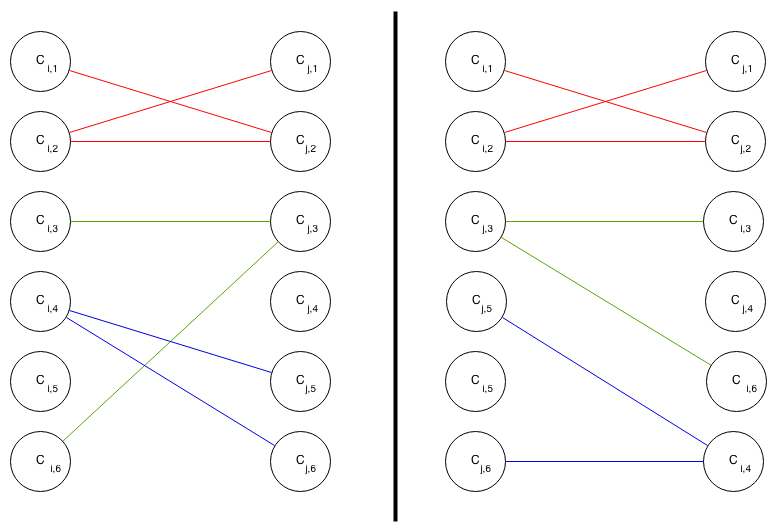
\includegraphics[height=10cm]{kempeSwap.png}\hfill
\centering

$t_i$\hspace{4.5cm}$t_j$\hspace{3.25cm}$t_i$\hspace{4.5cm}$t_j$ \\

\caption{Przykładowa zamiana łańcuchów Kempe: zielonego ($K_d$) i niebieskiego ($K_e$) dla okresów $t_i$ i $t_j$}
\label{fig:kempe_swap}
\end{figure}

\subparagraph{Przykład} 
Na rysunku \ref{fig:kempe_swap} po lewej stronie przedstawiono podgraf $G$, którego wierzchołkami są zajęcia, które zostały przydzielone do okresów $t_i$ i $t_j$, a krawędzie przedstawiają konflikty między kursami, do których należą te zajęcia. W podgrafie można wyróżnić 5 łańcuchów Kempe: $K_a = \{c_{i1}, c_{i2}, c_{j1}, c_{j2}\}$, $K_b = \{c_{i5}\}$, $K_c = \{c_{j4}\}$, $K_d = \{c_{i3}, c_{i6}, c_{j3}\}$, $K_e = \{c_{i4}, c_{j5}, c_{j6}\}$. Przykładowa zamiana dla łańcuchów $K_d$ i $K_e$ tworzy nowe przypasowanie (na rysunku \ref{fig:kempe_swap} po prawej stronie) przez przydzielenie $\{c_{i3}, c_{i4}, c_{i6}\}$ do $t_j$ i $\{c_{j3}, c_{i4}, c_{i6}\}$ do $t_i$.

\subparagraph{}Tak określony ruch można traktować jako rozszerzoną wersję podstawowej struktury sąsiedztwa, gdzie zamieniamy po kilka przypasowań na raz. Przy zamianie musimy uważać, aby nie wykonywać ruchów, które powodują przypasowanie do przedziałów czasowych większej liczby kursów, niż jest dostępnych sal. Dodatkowo nakładamy ograniczenia na liczbę kursów biorących udział w zamianie, tj. $|K_1|+ |K_2| \geq 3 $

%- room assignment
\par Po dokonaniu zamian w planie zajęć za pomocą łańcuchów Kempe następuje przypasowanie odpowiedniej sali do poszczególnych zajęć z danego okresu. Sale są przyporządkowywane do kursów metodą zachłanną, w każdym kroku wybieramy kurs, który nie ma przypisanej sali i jest kursem na który uczęszcza najwięcej studentów. Przypisujemy do kursu największą dostępną salę, sala zostaje oznaczona jako niedostępna.

\end{enumerate}
\paragraph{Lista tabu} służy do przechowywania informacji o ruchach tabu - ruchach, które nie mogą być wykonane przez określoną w tabu tenure dla kursu $c_{i}$ liczbę iteracji.
%-  dokłady opis tabu list
\subparagraph{}W przypadku sąsiedztwa prostego, jeśli zajęcia z kursu $c_i$ zostały przeniesione z okresu $t_j$ i sali $r_k$ w inne miejsce, wtedy przeniesienie jakichkolwiek zajęć z kursu $c_i$ do przedziału czasowego $t_j$ i sali $r_k$ przez kolejne $tt$ iteracji jest ruchem tabu. Podobnie dla sąsiedztwa zaawansowanego, jeśli zajęcia z kursu $c_i$ zostały przeniesione z przedziału czasowego $t_j$ do jakiegoś innego, wtedy przeniesienie jakichkolwiek zajęć z kursu $c_i$ do przedziału czasowego $t_j$ przez kolejne $tt$ iteracji jest ruchem tabu.\\

\subparagraph{Funkcja określająca liczbę iteracji, przez które ruch jest pamiętany na liście tabu} $tt(c_{i})$ obliczana jest na podstawie obecnie uzyskanego rozwiązania oraz częstotliwości przenoszenia zajęć z kursu $c_{i}$ oznaczonej przez $freq(c_{i})$. \\
Funkcję określono poniższym wzorem: 
 \[tt(c_{i}) = funkcja\ kary\ dla\ obecnego\ rozwiązania + \alpha * freq(c_{i}) \] 
gdzie ${\alpha = \frac{liczba\ konfliktujących\ kursów\ z\ c_{i}}{liczba\ kursów}}$ wobec tego wartość parametru ${\alpha \in [0, 1]}$ \\
gdyż ${liczba\ kursów \geq liczba\ konfliktujących\ kursów\ z\ c_{i}} $
\subparagraph{}Dzięki wprowadzeniu funkcji $tt(c_i)$ zróżnicowano czas, przez jaki różne ruchy są pamiętane na liście tabu. Ruchy wykonywane na początku przeszukiwania (kiedy funkcja kosztu jest wysoka) są pamiętane dłużej. Wprowadzenie czynnika zależnego od częstotliwości przenoszenia zajęć ma na celu przeciwdziałanie wielokrotnemu przenoszeniu zajęć tego samego kursu w to samo miejsce.

\paragraph{Procedura Tabu Search dla Adaptacyjnego Przeszukiwania Tabu}
\hfill
\begin{algorithm}[H]
    
    \begin{algorithmic}
    \STATE{$rozwiazanie_{najlepsze} = rozwiazanie_{aktualne}$}
    \WHILE{\emph{nie jest spełniony warunek stopu}}
    \STATE{$rozwiazanie_1 = tabu\_search\_proste\_sasiedztwo(rozwiazanie_{aktualne}, \theta)$}
    \STATE{$rozwiazanie_2 = tabu\_search\_zaawansowane\_sasiedztwo(rozwiazanie_1, \frac{\theta}{3})$}
    \IF	{$jakość(rozwiazanie_2)<jakość(rozwiazanie_{najlepsze})$}
    \STATE $rozwiazanie_{najlepsze} = rozwiazanie_2$
    \STATE $rozwiazanie_{aktualne} = rozwiazanie_2$
    \ENDIF

    \ENDWHILE
    \caption{Procedura $Tabu~search(rozwiazanie_{aktualne}, \theta)$}
    \label{tabusearch_tokenring}
    \end{algorithmic}
    \end{algorithm}
\par W algorytmie \ref{tabusearch_tokenring} $\theta$ oznacza głębokość przeszukiwania procedur $tabu\_search$ dla sąsiedztwa prostego i zaawansowanego.
\subsubsection{Faza dywersyfikacji}
\par Jeżeli rozwiązanie nie może zostać poprawione za pomocą algorytmu Tabu Search z \ref{tabusearch_tokenring} uruchamiana jest trzecia faza - faza dywersyfikacji. Głównym jej elementem jest losowy operator zaburzeń mający na celu opuszczenia osiągniętego lokalnego minimum. Początkowo identyfikowane są zajęcia z wysoką karą wynikającą z funkcji oceny  i losowo wybierane są zajęcia dla których zostaną dokonane zamiany sprecyzowane w poprzedniej fazie.
\par W momencie zakończenia fazy intensyfikacji, poszczególne zajęcia ustawiane są w kolejności malejącej ze względu na wysokość funkcji oceny. Z puli $q$ pierwszych zajęć wybierane jest $n$ zajęć, gdzie zajęcie będące na $k$ miejscu w rankingu wybierane zgodnie z normalizowanym rozkładem $P(k) = k^{-4.0}$. Następnie dokonywane jest $n$ losowych zamian pomiędzy zajęciami (sprecyzowanych w fazie intensyfikacji), ale tylko takich które zawierają przynajmniej jedno z wybranych z rankingu zajęć. \\
Przykład dla parametrów $q = 5$ i $n = 3$:
\begin{enumerate}
\item Po obliczeniu funkcji kary dla poszczególnych zajęć - ustawiamy zajęcia w kolejności nierosnącej pod względem funkcji kary (w $[\ ]$ podano przykładowe wartości funkcji kary)\\
\begin{enumerate}
 \item[(1)] $(t_{4}, fizyka, sala1)[127]$
 \item[(2)] $(t_{3}, religia, sala1)[89]$
 \item[(3)] $(t_{3}, język\ polski, sala2)[88]$
 \item[(4)] $(t_{4}, etyka, sala2)[80]$
 \item[(5)] $(t_{4}, język\ angielski, sala3)[77]$
 \item[(6)] $(t_{1}, język\ angielski, sala3)[52]$
 \item[(7)] $(t_{1}, biologia, sala2)[40]$
 \item[(8)] $(t_{2}, matematyka, sala2)[34]$
 \item[(9)] $(t_{2}, historia, sala1)[25]$
\end{enumerate}
\item Z puli wszystkich przedmiotów wybieramy $q = 5$ przedmiotów czyli przedmioty $(1) - (5)$ 
\item Rozkłady przed normalizacją dla wybranych $q$ zajęć:
	\begin{enumerate}
	\item[(1)] $P(1) = 1^{-4.0} = 1$
 	\item[(2)] $P(2) = 2^{-4.0} = \frac{1}{16}$
 	\item[(3)] $P(3) = 3^{-4.0} = \frac{1}{81}$
 	\item[(4)] $P(4) = 4^{-4.0} = \frac{1}{256}$
 	\item[(5)] $P(5) = 5^{-4.0} = \frac{1}{625}$
	\end{enumerate}
\item Losowane jest bez powtórzeń $n = 3$ zajęć zgodnie z powyższym rozkładem po dokonaniu normalizacji \\
	Przykłady wylosowanych zajęć [*]:
	\begin{enumerate}
	 \item[(1)] $(t_{4}, fizyka, sala1)[127]$
	 \item[(2)] $(t_{3}, religia, sala1)[89]$
	  \item[(4)] $(t_{4}, etyka, sala2)[80]$
	\end{enumerate}
\item Dla każdego z zajęć losujemy typ zamiany: podstawowa zamiana lub Kempe oraz znajdujemy wszystkie wykonywalne zamiany dla tego typu. Losowo wybieramy zamianę i przeprowadzamy ją. Odznaczając zajęcia, które są na liście [*], a dla których została już wykonana zamiana zawierająca te zajęcia.
\end{enumerate}




\subsection{Szczegóły implementacyjne}
\subsubsection{Struktury danych}
\paragraph{} Na potrzeby implementacji algorytmu plan zajęć został zamodelowany przy użyciu podstawowych struktur danych z języka Python. W pierwotnej wersji miał postać słownika, którego kluczami były kolejne numery przedziałów czasowych, a wartościami były listy, które przechowywały obiekty przypasowań zawierające identyfikatory kursu i sali. W trakcie implementacji okazało się, że kopiowanie takiej struktury wymaga korzystania z metody \verb#deepcopy# z modułu \verb#copy#, która przy wielu wywołaniach i dużej strukturze danych okazała się być nieefektywna. Ta obserwacja spowodowała, że w ostatecznej wersji obiekty przypasowań zastąpiono wbudowanym typem \verb#tuple#.
\subsubsection{Funkcja kosztu}
\paragraph{} Pomimo rozbudowanej matematycznej definicji funkcji kosztu w literaturze, efektywna implementacja okazała się być nietrywialna. Pierwsza wersja implementacji potrzebowała przejrzeć cały plan zajęć dla każdego ograniczenia miękkiego, w wersji ostatecznej wystarczą do tego tylko 2 przeglądy. Optymalizacja funkcji kosztu jest kluczowa dla czasu działania algorytmu. Korzystając z narzędzi do profilowania - moduł \verb#line_profile# - zauważyliśmy, że zdecydowaną większość czasu algorytm przeznacza na wykonanie funkcji kosztu.
\subsubsection{Optymalizacje językowe}
\paragraph{} Implementując algorytm staraliśmy się korzystać z funkcjonalnego paradygmatu programowania - funkcji \verb#map# i \verb#filter#, które w porównaniu ze zwykłymi pętlami w Pythonie nie mają dodatkowego narzutu przy iterowaniu. Ponadto korzystanie z elementów programowania funkcjonalnego spowodowało, że kod źródłowy jest w naszej ocenie bardziej zwięzły i czytelny.
\subsubsection{Test-Driven Development}
\paragraph{} Przy implementacji algorytmu staraliśmy wykorzystywać podejście TDD, czyli pisanie testów jednostkowych dla funkcji przed implementacją funkcji. ,,Szczelne'' pokrycie testami jednostkowymi podstawowych funkcji zdecydowanie ułatwiło późniejsze większe zmiany w logice i strukturze algorytmu.





\section{Particle Swarm Optimization (PSO)}
\author{Paweł Jastrzębski}
\subsection{Ogólny opis algorytmu}
\par Particle Swarm Optimaliation (PSO) lub optymalizacja rojem cząsteczek jest algorytmem zaproponowanym przez Jamesa Kennedy'ego oraz Russela Eberhart'a w roku 1995. Jest to technika wzorowana na zachowaniach występujących w przyrodzie. Algorytm naśladuje inteligencje i sposób poruszania się roju owadów poszukujących pożywienia. 
\par Zachowania te są w pewien sposób upraszczane, zamiast roju owadów mamy pewną liczbę cząsteczek (agentów) poruszających się w n-wymiarowej przestrzeni. Cząsteczki przemieszczają się w różnych kierunkach poszukując optymalnego rozwiązania. Korzystają przy tym ze swoich indywidualnych doświadczeń jak i doświadczenia ogółu.
\subsection{Działanie algorytmu}
\subsubsection{Oryginalna wersja}
\par W podstawowej wersji algorytmu używane są:
\begin{description}
  \item[Rój] \hfill \\
      Który posiada:
    \begin{itemize}
      \item Cząsteczki 
      \item Najlepszą pozycję (najlepsza pozycja osiągnięta dotychczas przez cząsteczki)
    \end{itemize}
  \item[Cząsteczki] \hfill \\
      Mające cechy:
    \begin{itemize}
      \item Pozycja (aktualna pozycja cząsteczki)
      \item Prędkość (wektor definiujący zmianę pozycji)
      \item Najlepsza pozycja (najlepsza pozycja osiągnięta przez tą konkretną cząsteczkę)
    \end{itemize}
\end{description}
\par Przebieg algorytmu można opisać poniższymi krokami:
\begin{description}
  \item[Krok 1:] 
     \par Stworzenie cząsteczek. Polega ono na ustawieniu ich pozycji i prędkości w sposób losowy. 
  \item[Krok 2:]
    \par Obliczenie prędkości dla każdej cząsteczki z osobna. 
  \item[Krok 3:]
        \par Zmiana pozycji każdej cząsteczki zgodnie z jej prędkością.
  \item[Krok 4:]
        \par Wyliczenie wartości funkcji dla aktualnych pozycji cząsteczek.
  \item[Krok 5:] 
      \par Sprawdzanie czy któraś cząsteczka poprawiła najlepszą pozycję roju lub samej siebie. Jeśli tak to aktualizujemy odpowiednią najlepszą pozycję.

\end{description}
    \par Kroki 2 - 5 są powtarzane aż do osiągnięcia wystarczająco dobrego wyniku lub maksymalnej liczby iteracji.
\subsubsection{PSO w problemie układania planu}
\par Modyfikacja PSO przedstawiona w tym rozdziale została zaczerpnięta z pracy ,,Timetable Scheduling Using Particle Swarm Optimization'' \cite{pso}
\par W tym podejściu każda cząsteczka posiada dwa kompletne plany zajęć. Jeden z nich jest przeznaczony do modyfikacji w każdej iteracji algorytmu (dalej nazywany planem aktualnym). Natomiast drugi plan jest używany do zapamiętywania dotychczas najlepszego planu znalezionego przez tą cząsteczkę (dalej nazywany lokalnie najlepszym planem). Obecny jest również globalny plan, którego zadaniem jest przechowywanie najlepszego planu znalezionego kiedykolwiek przez jakąkolwiek cząsteczkę (dalej nazywany globalnie najlepszym planem).  
\par Podczas każdej iteracji poszczególne cząsteczki będą poddawane trzem zmianom. Najpierw dwie losowe lekcje z planu aktualnego zostaną ze sobą zamienione. Potem jedna lekcja z lokalnie najlepszego planu zostanie skopiowana do aktualnego planu. Na koniec skopiujemy jedną lekcje z globalnie najlepszego planu do aktualnego planu. Kopia lekcji z innego planu wykonywana jest w następujący sposób. Wybierana jest lekcja z innego planu. Odszukujemy miejsce gdzie jest ta lekcja w aktualnym planie. Zamieniamy odszukaną lekcje z lekcją, która jest w miejscu do którego chcemy ją skopiować. 
\par Cały algorytm zaczynamy od stworzenia populacji dwudziestu cząsteczek. Każda z nich będzie posiadała losowo wygenerowany plan zajęć. Następnie dla każdej iteracji na każdej cząsteczce wykonywane będą poniższe kroki:
\begin{description}
  \item[Krok 1] \hfill \\
     \par Ocena rozwiązania. \hfill \\
   \par Oceniany zostaje aktualny plan. W tym momencie następuje aktualizacja lokalnie najlepszego planu oraz globalnie najlepszego planu.
  \item[Krok 2] \hfill \\
     \par Lokalna zamiana lekcji. \hfill \\
    \par Wykonana zostaje losowa zamiana dwóch lekcji w aktualnym planie.

  \item[Krok 3] \hfill \\
      \par Kopia lekcji z lokalnie najlepszego planu. \hfill \\
        \par Losowo wybrana lekcja z lokalnie najlepszego planu zostaje skopiowana do aktualnego planu 
  \item[Krok 4] \hfill \\
      \par Kopia lekcji z globalnie najlepszego planu. \hfill \\
        \par Losowo wybrana lekcja z globalnie najlepszego planu zostaje skopiowana do aktualnego planu 
\end{description}
\par Iteracje powtarzamy do czasu aż nie osiągniemy wystarczająco dobrego planu lub osiągniemy maksymalną liczbę iteracji albo skończy się nam limit czasu.
\subsection{Ścieżka dojścia do ostatecznego rozwiązania}
\subsubsection{Problem z proponowanym rozwiązaniem}
\par Podczas testowania proponowanego rozwiązania wystąpił problem. Algorytm wykazał się słabą skutecznością i nie był w stanie usunąć całkowicie problemów związanych z ograniczeniami "twardymi". Jak wiemy z rozdziału drugiego ograniczania "twarde" w ostatecznym rozwiązaniu nie mają prawa być łamane.
\par Aby algorytm brał pod uwagę w pierwszej kolejności ograniczenia "twarde", kary przydzielane za ich łamanie są mnożone przez milion.
Poniższy wykres pokazuje efektywność algorytmu. Uwagę należy zwrócić na skalę przyjętą na osi y. Wartości nie schodzą poniżej $10^{7}$ czyli wynik w najlepszym wypadku nadal łamie 10 ograniczeń "twardych".
\begin{figure}[H]
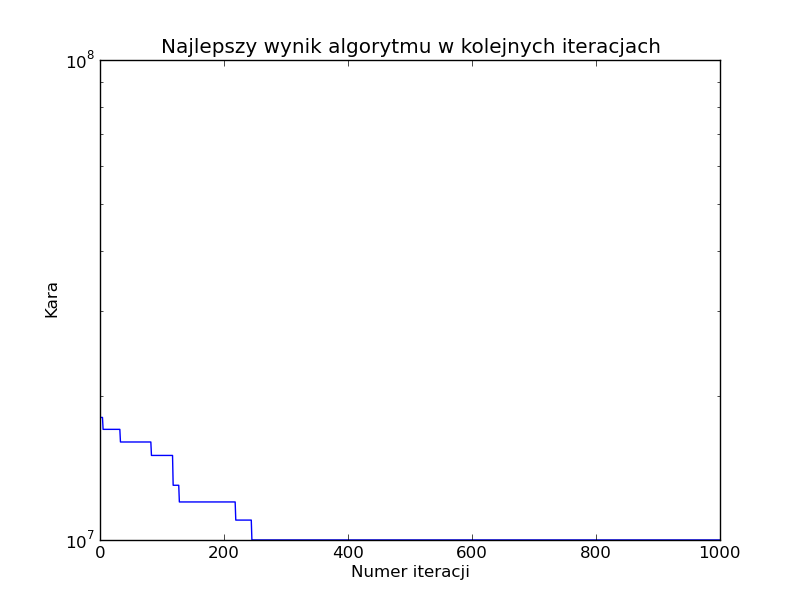
\includegraphics[width=10cm]{img/standard_penalty.png}
\centering
\end{figure}
\par Aby sprawdzić co się dzieje przyjrzałem się zachowaniu pojedynczej cząsteczki. Okazało się, że kara za kolejno generowane plany oscyluje wokół kary wyliczonej dla początkowego planu. Pokazuje to poniższy wykres.  
\begin{figure}[H]
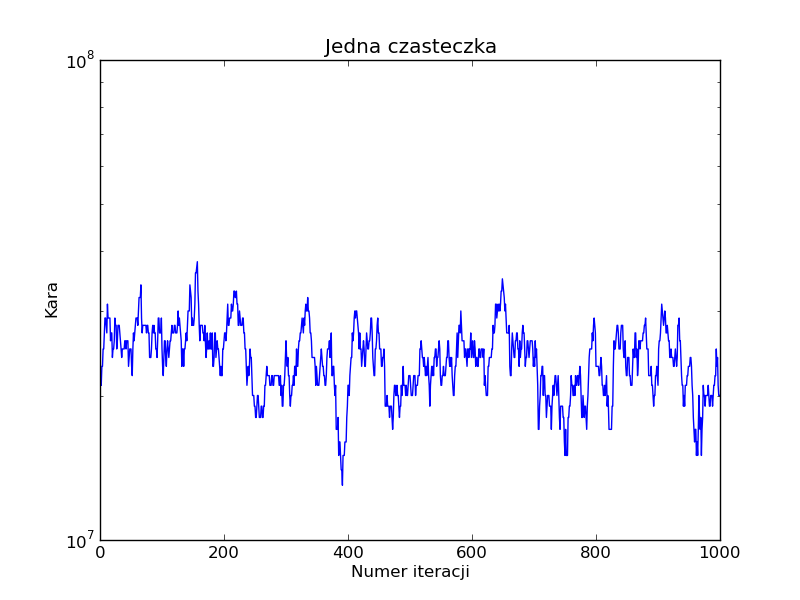
\includegraphics[width=10cm]{img/standard_particle.png}
\centering
\end{figure}
\par Na podstawie dalszej analizy okazało się, że wszystkie cząsteczki zachowują się bardzo podobnie. Widać to na poniższym wykresie.
\begin{figure}[H]
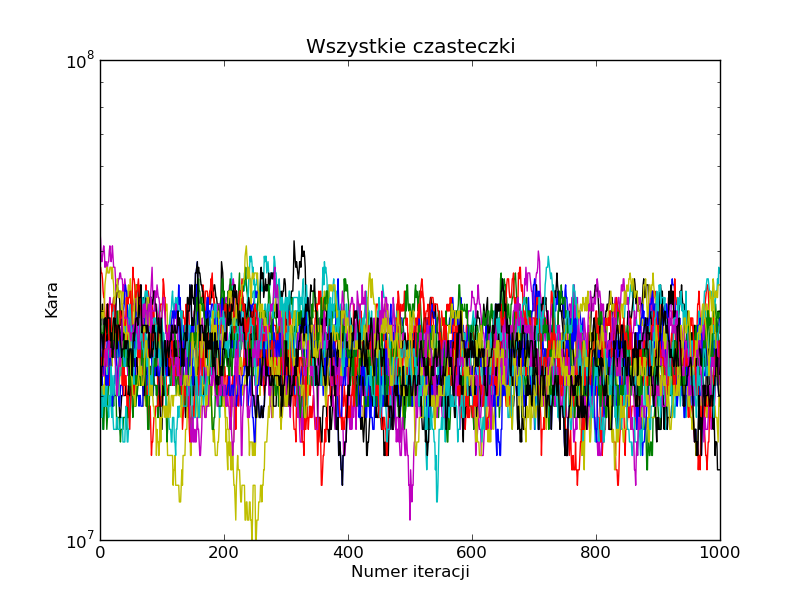
\includegraphics[width=10cm]{img/standard_particle_all.png}
\centering
\end{figure}
\subsubsection{Rozważane modyfikacje}
\par Rozważyłem dwie modyfikacje do aktualnego algorytmu. Jedną nazwałem podążaniem za lokalnie najlepszym planem, a drugą podążanie za globalnie najlepszym planem. Obie modyfikacje są względem siebie analogiczne, a różnią się tylko tym który plan bierzemy pod uwagę. Modyfikacją została objęta faza oceny aktualnego rozwiązania, która zachodzi na początku każdej iteracji. Dodany został warunek, że jeśli aktualny plan jest gorszy od najlepszego planu to zostaje on zamieniony na najlepszy plan. Usunięte też zostały kroki 3 i 4 czyli kopie z najlepszych planów.
\par W przypadku gdy każda cząsteczka podąża za swoim lokalnie najlepszym planem istnieje mniejsze ryzyko, że algorytm utknie w minimum lokalnym przestrzeni rozwiązań. Natomiast podczas podążania za globalnie najlepszym planem algorytm będzie znacznie szybciej dążył do najbliższego minimum.
\par Opcja podążania za lokalnie najlepszym planem okazała się być dużo efektywniejsza od podstawowego algorytmu. W tym przypadku ograniczenia "twarde" nie stanowiły problemu. Można to zobaczyć na poniższym wykresie.
\begin{figure}[H]
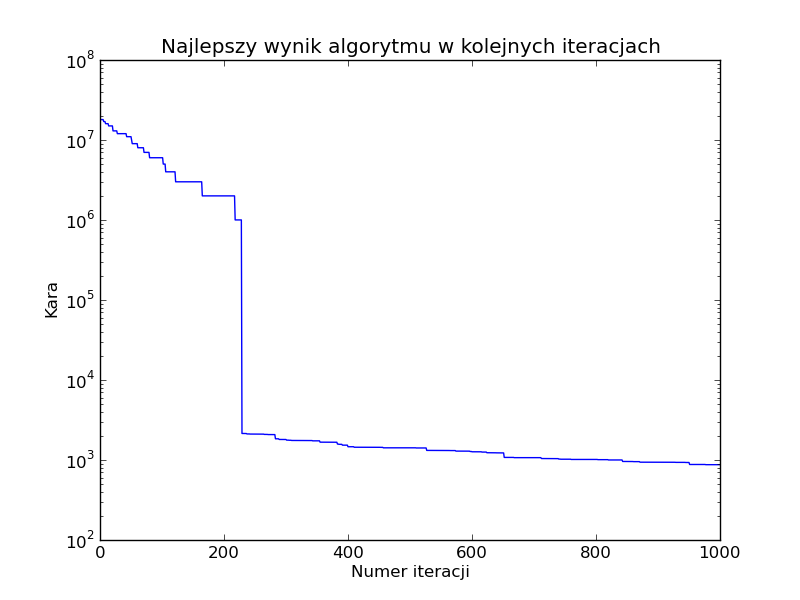
\includegraphics[width=10cm]{img/localbest_penalty.png}
\centering
\end{figure}
\par Analizując pojedynczą cząsteczkę można zauważyć, że często kara skacze od małych wartości do wartości milionowych. Jest to spowodowane tym, że w po zamianie dwóch lekcji w poprzedniej iteracji pojawił się konflikt z ograniczeniami "twardymi". Nie stanowi to problemu, ponieważ w takim przypadku wracamy do poprzedniego rozwiązania. Na poniższych wykresach widać zachowanie dla pojedynczej cząsteczki oraz dla wszystkich cząsteczek.
\begin{figure}[H]
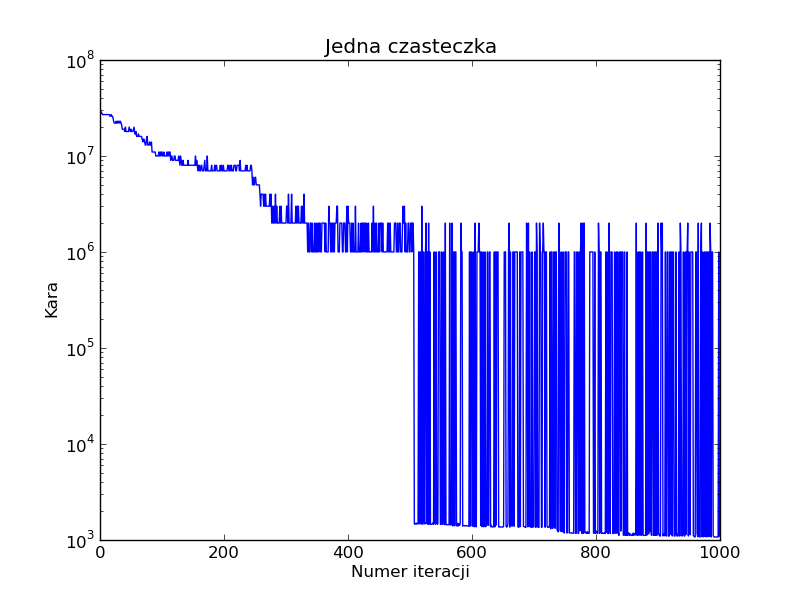
\includegraphics[width=10cm]{img/localbest_particle.png}
\centering
\end{figure}
\begin{figure}[H]
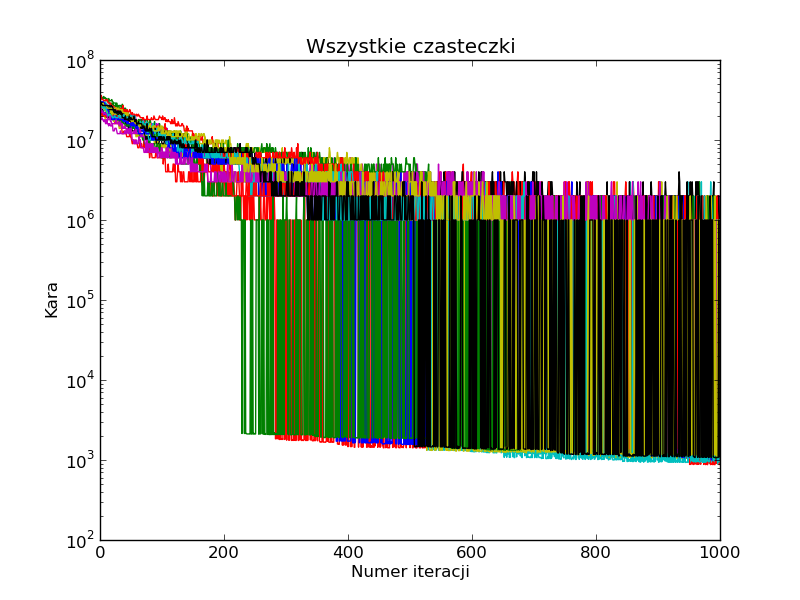
\includegraphics[width=10cm]{img/localbest_particle_all.png}
\centering
\end{figure}
\par Opcja podążania za globalnie najlepszym planem okazała się jeszcze bardziej efektywna. Sporym zaskoczeniem był brak problemów z lokalnymi minimami przestrzeni rozwiązań. Poniższy wykres pokazuje skuteczność modyfikacji.
\begin{figure}[H]
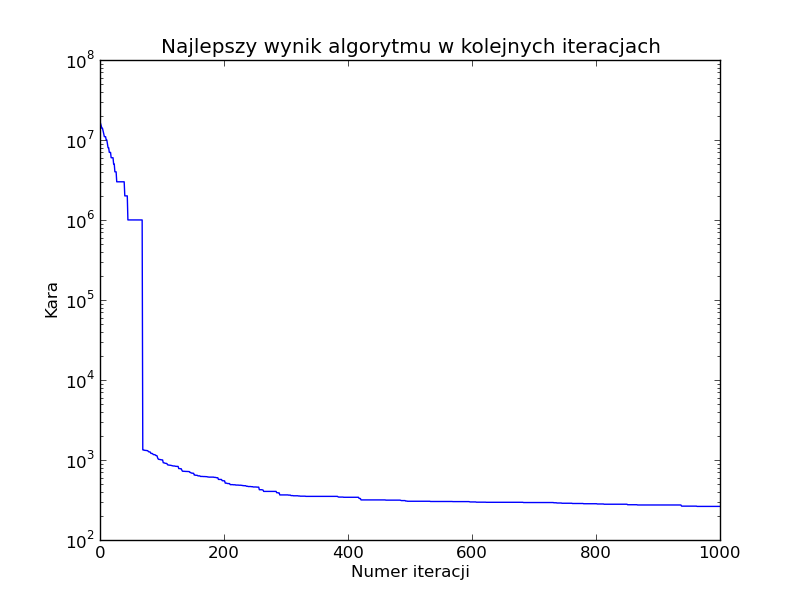
\includegraphics[width=10cm]{img/globalbest_penalty.png}
\centering
\end{figure}
\par W tym przypadku cząsteczki zachowywały się bardzo podobnie. Jedyną różnicą była prędkość z jaką spadała kara. Widać to na poniższych wykresach. 
\begin{figure}[H]
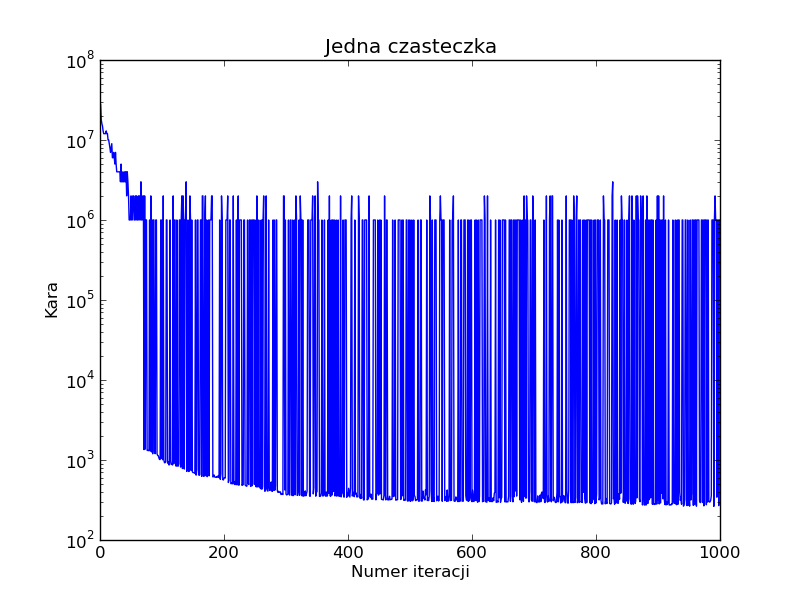
\includegraphics[width=10cm]{img/globalbest_particle.png}
\centering
\end{figure}
\begin{figure}[H]
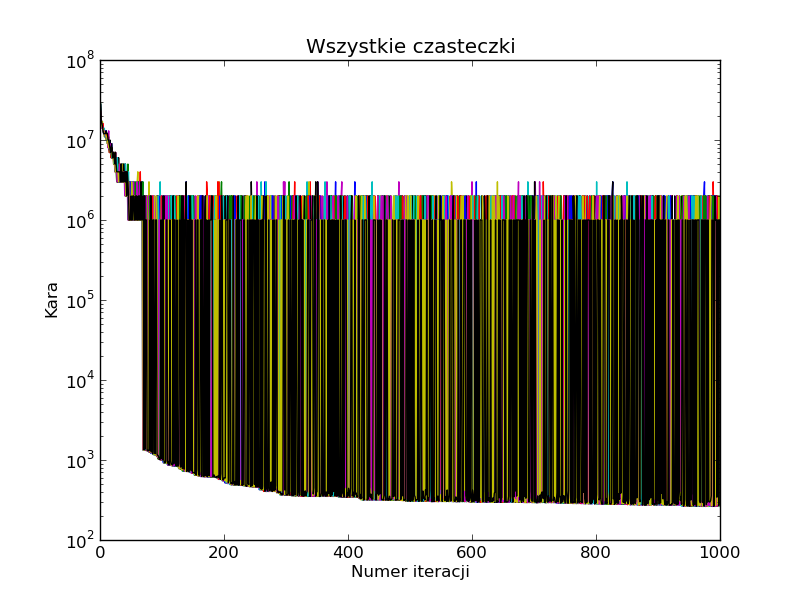
\includegraphics[width=10cm]{img/globalbest_particle_all.png}
\centering
\end{figure}
\subsubsection{Ostateczne rozwiązanie}
\par Jako ostateczne rozwiązanie wybrałem podążanie za globalnie najlepszym planem. Jest to spowodowane tym, że mimo wielu testów nie udało mi się znaleźć przypadku kiedy podążanie za lokalnie najlepszym planem wypadłoby lepiej. 


\section{Genetic Algorithm}
\author{Filip Czajkowski}
\subsection{Ogólny opis algorytmu}
\par Algorytm genetyczny to rodzaj algorytmu przeszukującego przestrzeń alternatywnych rozwiązań problemu w celu wyszukania rozwiązań najlepszych. Obecnie zalicza się go do grupy algorytmów ewolucyjnych.
\par Algorytmy genetyczne zajmują bardzo ważne miejsce w dziedzinie projektowania i analizy algorytmów. Doskonale sprawdzają się w sytuacji, gdy problem, z którym przychodzi nam się zmierzyć, jest nie do rozwiązania w sposób klasyczny w sensownym czasie. Pozwalają znaleźć sub-optymalne rozwiązanie problemów, których dziedziny nie są łatwe do wyznaczenia. Są powszechnie stosowane tam, gdzie do uzyskania rozwiązania korzystamy z zagadnień sztucznej inteligencji oraz tam, gdzie uzyskanie rozwiązania jest bardzo złożonym problem, natomiast jego ocena jest łatwa i błyskawiczna.
\par Należy zaznaczyć, że algorytm genetyczny nie gwarantuje znalezienia rozwiązania optymalnego, lecz przybliżone. Istota jego działania jest zbliżona do charakterystycznych dla środowiska naturalnego procesów ewolucyjnych. Cały algorytm operuje na grupie (populacji) potencjalnych rozwiązań, których jakość (stopień, w jakim jest bliskie rozwiązania optymalnego) potrafimy ocenić i które zbliżają się w przypominającym ewolucyjny procesie do rozwiązania optymalnego.
\par Problem definiuje środowisko, w którym istnieje pewna populacja osobników. Każdy z osobników ma przypisany pewien zbiór informacji stanowiących jego genotyp, a będących podstawą do utworzenia fenotypu. Fenotyp to zbiór cech podlegających ocenie funkcji przystosowania modelującej środowisko. Innymi słowy - genotyp opisuje proponowane rozwiązanie problemu, a funkcja przystosowania ocenia, jak dobre jest to rozwiązanie. Genotyp składa się z chromosomów, gdzie zakodowany jest fenotyp i ewentualnie pewne informacje pomocnicze dla algorytmu genetycznego. Chromosom składa się z genów.
\par Najczęściej działanie algorytmu przebiega następująco:
\begin{enumerate}
\item Losowana jest pewna populacja początkowa.
\item Populacja poddawana jest ocenie (selekcja). Najlepiej przystosowane osobniki biorą udział w procesie reprodukcji.
\item Genotypy wybranych osobników są ze sobą kojarzone poprzez złączanie genotypów rodziców (krzyżowanie).
\item Przeprowadzana jest mutacja, czyli wprowadzenie drobnych losowych zmian.
\item Rodzi się kolejne pokolenie. Aby utrzymać stałą liczbę osobników w populacji te najlepsze (według funkcji oceniającej fenotyp) są powielane, a najsłabsze usuwane. Jeżeli nie znaleziono dostatecznie dobrego rozwiązania, algorytm powraca do kroku drugiego. W przeciwnym wypadku wybieramy najlepszego osobnika z populacji - jego genotyp to uzyskany wynik.
\end{enumerate}
\subsection{Historia i zastosowanie}
Sposób działania algorytmów genetycznych nieprzypadkowo przypomina zjawisko ewolucji biologicznej, ponieważ ich twórca John Henry Holland właśnie z biologii czerpał inspiracje do swoich prac. 
\subsection{Fazy algorytmu}
\subsubsection{Utworzenie rozwiązania początkowego}
\subsubsection{Selekcja}
\subsubsection{Krzyżowanie}
\subsubsection{Mutacja}
\subsubsection{Elityzm}
\subsection{Istniejące implementacje}
\chapter{Projekt systemu}
\subsection{Zastosowanie}
\subsubsection{Przypadki użycia}
\par
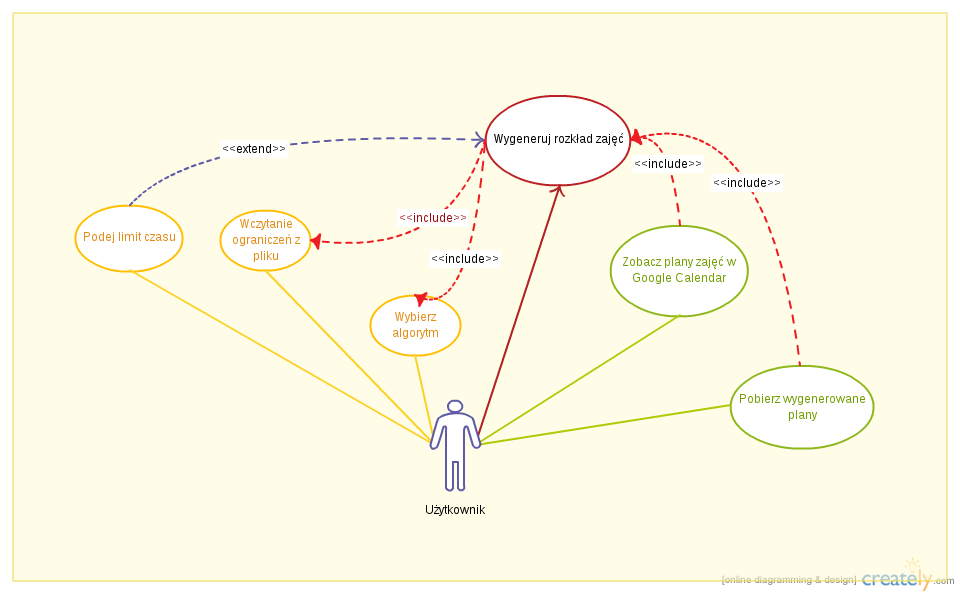
\includegraphics[width=0.8\textwidth]{InzynierkaUseCase.png}
\subsection{Architektura systemu}

\par
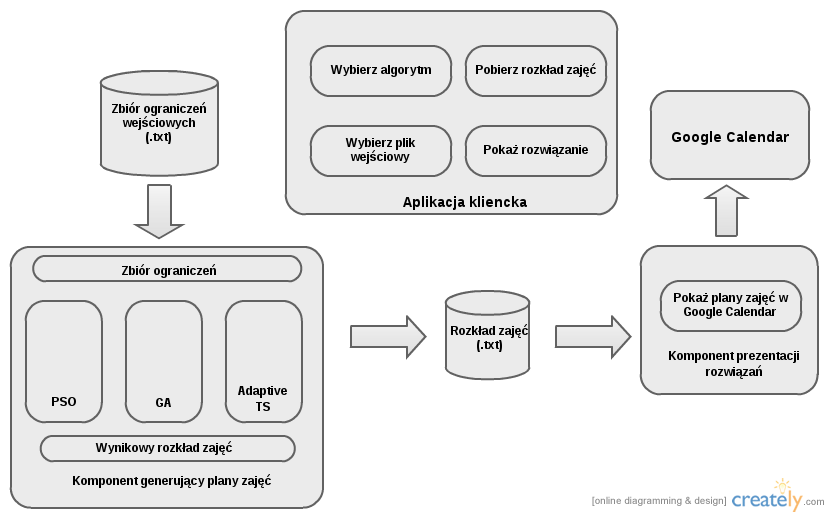
\includegraphics[width=0.8\textwidth]{ComponentsDiagram.png}
\subsection{Rozwiązania implementacyjne}
\chapter{Testy i porównanie algorytmów}

\chapter{Sposób użytkowania systemu}
\chapter{Podsumowanie}

\begin{thebibliography}{2}
\bibitem{tabu} Zhipeng Lu, Jin-Kao Hao. Adaptive TabuSearch for Course Timetabling.  \emph{European Journal of Operational Research}, 200(1):235-244, 2010.
\bibitem{com} U. Brannlund, P. ). Lindberg, A. Nou, J. E. Nilsson. Timetabling using lagrangian relaxation Transportation Science 32, 358-369, 1998
\bibitem{sport} J. A. M. Schreuder. Constructing timetables for sport competitions. \emph{Mathematical Programming Study 13}, 58-67, 1980
\bibitem{worker} M. Chiarandini, A. Schaerf, F. Tiozzo. Solving employee timetabling problems with flexible workload using tabu search. \emph{Proceedings of the 3rd PATAT Conference}, 2013
\bibitem{pso} Autor1, Autor1. Tytuł.  \emph{European Journal of Operational Research}, 200(1):235-244, 2010.

\bibitem{glover} Fred Glover (1986). ,,Future Paths for Integer Programming and Links to Artificial Intelligence'' \emph{Computers and Operations Research}, 13 (5): 533–549.

\end{thebibliography}

\end{document}
